\setcounter{section}{0}
\section{Lý thuyết}
\subsection{Gia tốc hướng tâm}
\begin{center}
	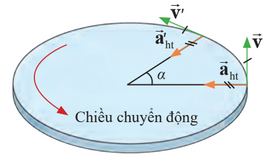
\includegraphics[scale=1]{../figs/G10-027-1}
	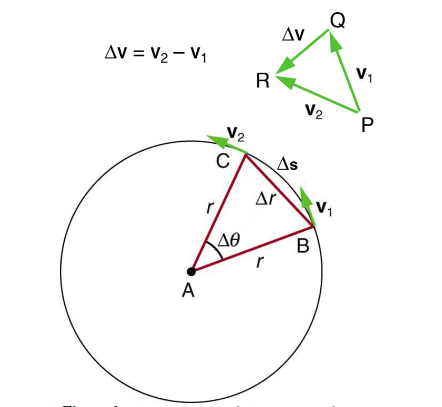
\includegraphics[height=5cm]{../figs/G10-027-1b}
\end{center}

\begin{itemize}
	\item Trong chuyển động tròn đều, vectơ gia tốc $\vec{a}=\Delta\vec{v}/\Delta t$  hướng vào  tâm đường tròn.
	\item Vectơ gia tốc hướng tâm đặc trưng cho sự biến đổi của vectơ vận tốc, kí hiệu là $\vec{a}_{ht}$.
	\item Độ lớn của vectơ gia tốc hướng tâm:
	\begin{equation*}
		a_\text{ht}=\frac{v^2}{r}=\omega^2 \cdot r.
	\end{equation*}
\end{itemize}
\subsection{Lực hướng tâm}
\begin{center}
	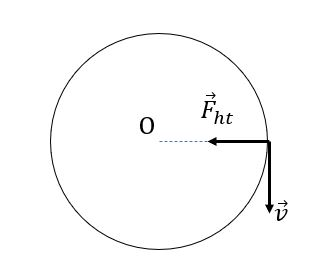
\includegraphics[scale=0.6]{../figs/VN10-PH-16-L-013-1-V2-04.JPG}
\end{center}
\subsubsection{Định nghĩa}
Lực (hay hợp lực của các lực) tác dụng vào một vật chuyển động tròn đều và gây ra cho vật gia tốc hướng tâm gọi là lực hướng tâm.
\subsubsection{Biểu thức}

\begin{equation*}
	F_{\text{ht}} = m \cdot a_{\text{ht}} = m\dfrac{v^2}{r},
\end{equation*}
trong đó:
\begin{itemize}
	\item $m$ là khối lượng của vật (kg), 
	\item $v$ là tốc độ dài của vật (m/s),
	\item $r$ là bán kính quỹ đạo (m),
	\item $F_{\text{ht}}$ là lực hướng tâm (N).
\end{itemize}

\subsection{Chuyển động li tâm}
\subsubsection{Thế nào là chuyển động li tâm?}
Xét ví dụ, ta đặt một vật trên bàn quay. 
\begin{itemize}
	\item Để giữ cho vật vẫn quay tròn đều cùng với bàn, cần có một lực hướng tâm. Lực ma sát nghỉ giữa vật và bàn chính là lực hướng tâm đó. 
	\item Nếu ta tăng tốc của bàn, lực hướng tâm cần thiết sẽ tăng lên (lực hướng tâm tỉ lệ với bình phương vận tốc). Lực ma sát nghỉ cũng tăng theo để đóng vai trò lực hướng tâm. 
	\item Nếu tăng tốc bàn đến một giá trị nào đó, lực hướng tâm cần thiết sẽ vượt quá giới hạn của lực ma sát nghỉ, khí đó lực ma sát nghỉ không còn giữ được vật trên quỹ đạo tròn. Vật sẽ bị trượt và văng ra khỏi quỹ đạo tròn theo phương tiếp tuyến với quỹ đạo. Chuyển động như vậy gọi là chuyển động li tâm.  
\end{itemize}

\subsubsection{Ứng dụng của chuyển động li tâm}
\begin{itemize}
	\item Máy vắt li tâm: ứng dụng trong máy giặt để vắt sạch nước trong quần áo, máy ép nước trái cây…
	\item Chuyển động li tâm dễ gây ra tai nạn khi các phương tiện chuyển động qua đoạn đường cong.
\end{itemize}
\subsection{Vật chuyển động tròn trên mặt phẳng thẳng đứng}
Chọn chiều dương là chiều hướng tâm.
\subsubsection{Áp lực tại điểm cao nhất và điểm thấp nhất}
\begin{itemize}
	\item Tại điểm cao nhất, áp lực có giá trị:
	\begin{equation*}
		F_\text{ht}=N+P\Rightarrow	N=-P + F_{\text{ht}}= -mg + \dfrac{mv^2}{r}.
	\end{equation*}
	\item Tại điểm thấp nhất, áp lực có giá trị:
	\begin{equation*}
		F_\text{ht}=N-P\Rightarrow	N = P + F_{\text{ht}} = mg + \dfrac{mv^2}{r}.
	\end{equation*}
\end{itemize}
\subsubsection{Lực căng dây tại điểm cao nhất và điểm thấp nhất}
\begin{itemize}
	\item Lực căng dây khi vật ở vị trí cao nhất:
	\begin{equation*}
		P+T=F_{\text{ht}} \Rightarrow T = F_\text{ht} - P = \dfrac{mv^2}{r} - mg.
	\end{equation*}
	\item Lực căng dây khi vật ở vị trí thấp nhất:
	\begin{equation*}
		-P+T = F_{\text{ht}} \Rightarrow T = F_\text{ht} + P = \dfrac{mv^2}{r} + mg.
	\end{equation*}
\end{itemize}
\section{Mục tiêu bài học - Ví dụ minh họa}
\begin{dang}{Tính gia tốc hướng tâm trong chuyển động tròn đều}
	
	\viduii{2}{Một vệ tinh nhân tạo ở độ cao $250\ \text{km}$ bay quanh Trái Đất theo một quỹ đạo tròn. Chu kì của vệ tinh là $88\ \text{phút}$. Tính gia tốc hướng tâm của vệ tinh. Cho bán kính Trái Đất là $6400\ \text{km}$
	}
	{	\begin{center}
			\textbf{Hướng dẫn giải}
		\end{center}
		
		Khoảng cách từ vệ tinh đến tâm Trái Đất: 
		$$r=250\ \text{km}+6400\ \text{km} =6650\ \text{km}=6650000\ \text{m}. $$
		Tốc độ góc của vệ tinh:
		$$T=\frac{2\pi}{\omega} \Rightarrow \omega = \frac{\pi}{2640}\ \text{rad/s}.$$ 
		Gia tốc hướng tâm của vệ tinh: 
		
		$$a_{ht}=\omega^2 \cdot r \approx \SI{9,41}{ \meter/\second^2}.$$ 
		
	}
	
	\viduii{2}{Một vật chuyển động theo đường tròn bán kính $r = \SI{100}{cm}$ với gia tốc hướng tâm $a_\text{ht} = \SI{4}{cm/s}^2$. Tính chu kì của chuyển động.
		
	}
	{	\begin{center}
			\textbf{Hướng dẫn giải}
		\end{center}
		
		Tốc độ dài của chuyển động
		$$a_\text{ht} =\dfrac{v^2}{r} \Rightarrow v =\sqrt {ra_\text{ht}}.$$
		
		Chu kì của chuyển động là
		$$T =\dfrac{2\pi}{\omega} = \dfrac{2\pi r}{v} = 2\pi \sqrt{\dfrac{r}{a_\text{ht}}} \approx \SI{31.415}{\second}.$$
		
	}
\end{dang}
\begin{dang}{Ghi nhớ công thức tính lực hướng tâm, đặc điểm của lực hướng tâm}
	\viduii{1}{Lực nào sao đây có thể là lực hướng tâm?
		\begin{mcq}(2)
			\item Lực ma sát.
			\item Lực hấp dẫn.
			\item Lực đàn hồi.
			\item Cả 3 đáp án trên.
		\end{mcq}
	}
	{	\begin{center}
			\textbf{Hướng dẫn giải}
		\end{center}
		
		Cả 3 lực trên đều có thể là lực hướng tâm.
		
		\textbf{Đáp án: D}.
	}
	\viduii{1}{Chọn phát biểu sai về lực hướng tâm:
		\begin{mcq}
			\item Vệ tinh nhân tạo chuyển động tròn đều quanh Trái Đất do lực hấp dẫn đóng vai trò lực hướng tâm.
			\item Xe chuyển động vào một đoạn đường cong (khúc cua), lực đóng vai trò hướng tâm luôn là lực ma sát.
			\item Xe chuyển động đều trên đỉnh một cầu võng, hợp lực của trọng lực và phản lực vuông góc đóng vai trò lực hướng tâm.
			\item Vật nằm yên đối với mặt bàn nằm ngang đang quay đều quanh trục thẳng đứng thì lực ma sát nghỉ đóng vai trò lực hướng tâm.
		\end{mcq}
	}
	{	\begin{center}
			\textbf{Hướng dẫn giải}
		\end{center}
		
		Nếu mặt đường nghiêng vào trong tâm quỹ đạo cong thì hợp lực của phản lực $N$ và trọng lực $P$ khi xe qua đoạn đường cong cũng đóng góp vào lực hướng tâm, không phải chỉ có lực ma sát.
		
		\textbf{Đáp án: B}.
	}
	\viduii{1}{Một vậy có khối lượng $m$ đang chuyển động tròn đều trên một quỹ đạo bán kính $r$ với tốc độ góc $\omega$. Lực hướng tâm tác dụng vào vật
		\begin{mcq}(2)
			\item $F_\text{ht} = m\omega^2 r.$
			\item $F_\text{ht} = \dfrac{mr}{\omega}.$
			\item $F_\text{ht} = \omega^2 r.$
			\item $F_\text{ht} = m\omega^2 .$
		\end{mcq}
	}
	{	\begin{center}
			\textbf{Hướng dẫn giải}
		\end{center}
		
		Lực hay hợp lực của các lực tác dụng lên một vật chuyển động tròn đều và gây ra cho vật gia tốc hướng tâm gọi là lực hướng tâm.
		
		$$F_\text{ht} = ma_\text{ht} = m\dfrac{v^2}{r} = m\omega^2 r.$$
		
		\textbf{Đáp án: A}.
	}
	
\end{dang}
\begin{dang}{Xác định lực hướng tâm}
	\viduii{3}{Lấy $g=\SI{10}{m/s^2}$. Tính áp lực của ô tô 4 tấn đi qua điểm giữa cầu với tốc độ $\SI{72}{km/h}$ trong các trường hợp sau:
		
		a) Cầu phẳng.
		
		b) Cầu cong lồi bán kính $\SI{100}{m}$.
		
		c) Cầu cong lõm bán kính $\SI{200}{m}$.
	}
	{	\begin{center}
			\textbf{Hướng dẫn giải}
		\end{center}
		
		\begin{itemize}
			\item Trọng lực $P$ và phản lực $N$ của mặt cầu đóng vai trò lực hướng tâm 
			\begin{equation*}
				\vec{F}_{\text{ht}} = \vec{P} +\vec{N}.
			\end{equation*}
			\item Xét về độ lớn phản lực $N$ cân bằng với áp lực của ô tô nén lên mặt cầu nên về mặt tính toán ta coi $N$ chính là độ lớn áp lực của ô tô lên mặt cầu.
		\end{itemize}
		a) Cầu phẳng, bán kính xem như rất lớn $r\to \infty$
		\begin{align*}
			F_\text{ht}=m\dfrac{v^2}{r}\to0.
		\end{align*}
		\begin{center}
			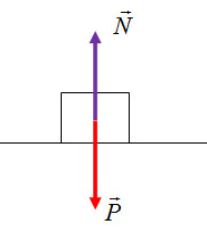
\includegraphics[scale=0.5]{../figs/VN10-PH-16-L-013-1-V2-01.JPG}
		\end{center}
		\begin{equation*}
			F_{\text{ht}} =0; N=P=mg=40000\ \text{N}.
		\end{equation*}
		b) Cầu cong lồi
		\begin{center}
			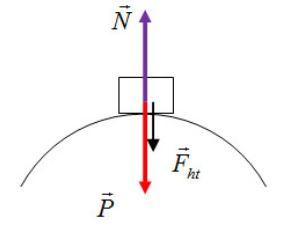
\includegraphics[scale=0.5]{../figs/VN10-PH-16-L-013-1-V2-02.JPG}
		\end{center}
		\begin{equation*}
			F_{\text{ht}} =P-N\Rightarrow  N=P-F_{\text{ht}} =mg-m\dfrac{v^2}{r}=24000\ \text{N}.
		\end{equation*}
		c) Cầu cong lõm
		\begin{center}
			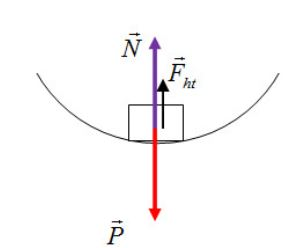
\includegraphics[scale=0.5]{../figs/VN10-PH-16-L-013-1-V2-03.JPG}
		\end{center}
		\begin{equation*}
			-F_{\text{ht}} =P-N\Rightarrow  N=P+F_{\text{ht}} =mg+m\dfrac{v^2}{r}=56000\ \text{N}.
		\end{equation*}
	}
	\viduii{3}{Một xe có khối lượng $m$ chuyển động trên đường cua tròn có bán kính $r = \SI{100}{m}$ với vận tốc không đổi $\SI{72}{km/h}$. Lấy $g = \SI{10}{m/s^2}$. Hệ số ma sát giữa lốp xe và mặt đường ít nhất bằng bao nhiêu để xe không trượt?
	}
	{	\begin{center}
			\textbf{Hướng dẫn giải}
		\end{center}
		
		Đổi đơn vị $\SI{72}{km/h}=\SI{20}{m/s}$.
		
		Xe chuyển động tròn đều nên lực ma sát nghỉ đóng vai trò là lực hướng tâm.
		
		Để xe không trượt trên đường thì:
		
		$$F_\text{ht} \leq F_\text{msn} \Rightarrow m\dfrac{v^2}{r} \leq \mu mg.$$
		
		$$\Rightarrow \mu \geq \dfrac{v^2}{gr} = \SI{0,4}{}\Rightarrow \mu_\text{min} =\SI{0,4}{}$$
	}
	%\end{dang}
	%\begin{dang}{Xác định lực hướng tâm \\là hợp lực của trọng lực và phản lực }
	\viduii{3}{Một xô nước coi như chất điểm có khối lượng tổng cộng là $\SI{2}{kg}$ được buộc vào sợi dây dài $\SI{0,8}{m}$. ta quay dây với vận tốc góc 45 vòng/phút trong mặt phẳng đứng. Tính lực căng của dây khi xô đi qua điểm cao nhất và điểm thấp nhất của quỹ đạo.
	}
	{	\begin{center}
			\textbf{Hướng dẫn giải}
		\end{center}
		
		\begin{itemize}
			\item Lực căng dây ở vị trí cao nhất:
			\begin{equation*}
				P+T =F_{\text{ht}} \Rightarrow T = m(\omega^2R -g)=\SI{15,9}{N}.
			\end{equation*}
			\item Lực căng dây ở vị trí thấp nhất: 
			\begin{equation*}
				-P+T =F_{\text{ht}} \Rightarrow T = m(\omega^2R +g)=\SI{55,1}{N}.
			\end{equation*}
		\end{itemize}
	}
	\viduii{4}{Một máy bay thực hiện vòng nhào lộn bán kính $\SI{400}{m}$ trong mặt phẳng đứng với vận tốc $\SI{540}{km/h}$. Lấy $g = \SI{10}{m/s^2}$.
		
		a) Tính lực do người lái có khối lượng $\SI{60}{kg}$ nén lên ghế ngồi ở điểm cao nhất và thấp nhất của vòng nhào lộn.
		
		b) Vận tốc máy bay phải bằng bao nhiêu để người lái không nén lên ghế?
	}
	{	\begin{center}
			\textbf{Hướng dẫn giải}
		\end{center}
		
		a) Tính lực do người lái có khối lượng $\SI{60}{kg}$ nén lên ghế ngồi ở điểm cao nhất và thấp nhất của vòng nhào lộn.
		
		\begin{itemize}
			\item Tại điểm thấp nhất áp lực của người lái nén lên ghế ngồi là
			\begin{equation*}
				N=P+F_{\text{ht}} = mg +\dfrac{mv^2}{R} = \SI{3975}{N}.
			\end{equation*} 
			\item Tại điểm cao nhất áp lực của người lái nén lên ghế ngồi là
			\begin{equation*}
				N=-P+F_{\text{ht}} = -mg +\dfrac{mv^2}{R} = \SI{2775}{N}.
			\end{equation*} 
		\end{itemize}
		
		b) Vận tốc máy bay phải bằng bao nhiêu để người lái không nén lên ghế?
		
		Để người lái không nén lên ghế thì $N=0$, suy ra 
		\begin{equation*}
			F_{\text{ht}}=P \Leftrightarrow mg = \dfrac{mv^2}{R} \Rightarrow v =\sqrt {gR} = 20\sqrt {10}\ \text{m/s}.
		\end{equation*}
	}
	\viduii{4}{Diễn viên xiếc đi xe đạp trên vòng xiếc bán kính $\SI{6,4}{m}$. Lấy $g = \SI{10}{m/s^2}$. Để đi qua điểm cao nhất mà không rơi thì người đó phải đi với tốc độ tối thiểu bằng bao nhiêu?
	}
	{	\begin{center}
			\textbf{Hướng dẫn giải}
		\end{center}
		
		Tại điểm cao nhất của vòng xiếc có các lực tác dụng lên xe là trọng lực $\vec P$ và phản lực  $\vec N$ của vòng xiếc.	
		
		$$P + N = F_\text{ht} = m \dfrac{v^2}{R} \Rightarrow N  =  m \dfrac{v^2}{R} - P =m \dfrac{v^2}{R}-mg .$$
		
		Muốn không bị rơi khỏi vòng xiếc thì vẫn còn lực ép lên vòng xiếc. Khi đó $N \geq 0 $, suy ra
		
		$$ m \dfrac{v^2}{R}-mg \geq 0 \Rightarrow v \geq \sqrt{gR} = 8 \Rightarrow v_\text{max} = \SI{8}{m/s}.$$
		
		
	}
	\viduii{4}{Một máy bay thực hiện một vòng bay trong mặt phẳng thẳng đứng. Bán kính vòng bay là $R= \SI{500}{m}$, vận tốc máy bay có độ lớn không đổi $v=\SI{360}{km/h}$. Khối lượng của người phi công là $m=\SI{75}{kg}$. Lấy $g=\SI{10}{m/s^2}$. Xác định lực nén của người phi công lên ghế ngồi tại điểm cao nhất và thấp nhất của vòng bay.
	}
	{	\begin{center}
			\textbf{Hướng dẫn giải}
		\end{center}
		
		Áp lực tại vị trí cao nhất:
		
		$$N_\text{A} = F_\text{q} - P = m \dfrac{v^2}{R} - mg =\SI{750}{N}.$$
		
		Áp lực tại vị trí thấp nhất:
		
		$$N_\text{B} = F_\text{q} + P = m \dfrac{v^2}{R} + mg =\SI{2250}{N}.$$
		
	}
\end{dang}


\section{Trắc nghiệm}
\begin{enumerate}[label=\bfseries Câu \arabic*:]

	\item \mkstar{2}
	
	
	{
		Một chất điểm chuyển động tròn đều với chu kì $T$, bán kính $R$. Công thức tính gia tốc hướng tâm của vật là
		\begin{mcq}(4)
			\item $a=4 \pi ^2 \dfrac{R^2}{T^2}$.
			\item $a=4 \pi \dfrac{R}{T^2}$.
			\item $a=4 \pi ^2 \dfrac{R}{T^2}$.
			\item $a=4 \pi ^2 \dfrac{R}{T}$.
		\end{mcq}
	}
	
	\hideall
	{	
		\textbf{Đáp án: C.}
		
		Gia tốc hướng tâm:
		$$a=\omega^2 R = \left(\dfrac{2\pi}{T}\right)^2 R = 4 \pi ^2 \dfrac{R}{T^2}$$
	}
	\item \mkstar{2}
	
	
	{
		Một vật đang chuyển động tròn đều dưới tác dụng của lực hướng tâm $F$. Nếu bán kính quỹ đạo tăng gấp hai lần so với trước và đồng thời giảm tốc độ quay còn một nửa thì so với ban đầu, lực hướng tâm
		\begin{mcq}(2)
			\item giảm 8 lần.
			\item giảm 4 lần.
			\item giảm 2 lần.
			\item không thay đổi.
		\end{mcq}
	}
	
	\hideall
	{	
		\textbf{Đáp án: A.}
		
		Ta lập tỉ lệ:
		$$\dfrac{F_\text{ht 1}}{F_\text{ht 2}} = \dfrac{v_1 ^2 r_2}{v_2 ^2 r_1} = 8$$
		
		Vậy lực hướng tâm giảm 8 lần.
	}
	\item \mkstar{2}
	
	
	{
		Khi ô tô chuyển động đều trên một đoạn đường có dạng cung tròn, lực tác dụng đóng vai trò lực hướng tâm là
		\begin{mcq}
			\item trọng lực của ô tô.
			\item phản lực của mặt đường.
			\item hợp lực của tất cả các lực tác dụng lên xe.
			\item lực ma sát giữa bánh xe và mặt đường.
		\end{mcq}
	}
	
	\hideall
	{	
		\textbf{Đáp án: C.}
		
		Khi ô tô chuyển động đều trên một đoạn đường có dạng cung tròn, lực tác dụng đóng vai trò lực hướng tâm là hợp lực của tất cả các lực tác dụng lên xe.
	}
	\item \mkstar{2}
	
	
	{
		Một đĩa tròn nằm ngang có thể quay quanh một trục thẳng đứng. Vật $m=\SI{100}{g}$ đặt trên đĩa, nối với trục quay bởi một lò xo nằm ngang. Nếu số vòng quay không quá $\omega_1 = 2\ \text{vòng/s}$ thì lò xo không biến dạng. Nếu số vòng quay tăng dần đến $\omega_2 = 5\ \text{vòng/s}$ thì lò xo dãn gấp đôi. Tính độ cứng $k$ của lò xo.
		\begin{mcq}(4)
			\item $\SI{182}{N/m}$.
			\item $\SI{232}{N/m}$.
			\item $\SI{419}{N/m}$.
			\item $\SI{336}{N/m}$.
		\end{mcq}
	}
	
	\hideall
	{	
		\textbf{Đáp án: A.}
		
		Đổi $\omega_1=\xsi{4\pi}{rad/s}$, $\omega_2 = \xsi{10\pi}{rad/s}$
		
		Khi lò xo chưa biến dạng:
		$$F_\text{ms} = F_\text{ht} = m \omega_1 l_0$$
		
		Khi lò xo biến dạng dãn gấp đôi:
		$$F_\text{ht} = F_\text{đh} + F-\text{ms} \Rightarrow m \omega_2 ^2 2l_0 = k (2l_0 - l_0) + m \omega_1 l_0 \Rightarrow k = m(2\omega_2 - \omega_1) = \SI{182}{N/m}$$
	}
	
	\item \mkstar{2}
	
	
	{
		Hai quả cầu $m_1=2m_2$ nối với nhau bằng dây dài $l=\SI{12}{cm}$ có thể chuyển động không ma sát trên một trục nằm ngang qua tâm của hai quả cầu. Cho hệ quay đều quanh trục thẳng đứng. Biết hai quả cầu đứng yên không trượt trên trục ngang. Tìm khoảng cách từ hai quả cầu đến trục quay.
		\begin{mcq}(2)
			\item $r_1=\SI{5}{}$, $r_2=\SI{8}{cm}$.
			\item $r_1=\SI{4}{}$, $r_2=\SI{8}{cm}$.
			\item $r_1=\SI{4}{}$, $r_2=\SI{6}{cm}$.
			\item $r_1=\SI{4}{}$, $r_2=\SI{10}{cm}$.
		\end{mcq}
	}
	
	\hideall
	{	
		\textbf{Đáp án: B.}
		
		Các quả cầu chuyển động quanh trục có khoảng cách đến tâm khác nhau, nhưng tốc độ góc thì vẫn như nhau. Lực căng dây đóng vai trò lực hướng tâm.
		
		Ta có:
		$$m_1 \omega^2 r_1 = m_2 \omega^2 r_2 \Rightarrow m_1 r_1 = m_2 r_2$$
		
		Mà $$r_1+r_2 = l$$
		
		Suy ra: $r_1 = \SI{4}{cm}$, $r_2 = \SI{8}{cm}$.		
	}
\end{enumerate}
\hideall
{
	\begin{center}
		\textbf{BẢNG ĐÁP ÁN}
	\end{center}
	\begin{center}
		\begin{tabular}{|m{2.8em}|m{2.8em}|m{2.8em}|m{2.8em}|m{2.8em}|m{2.8em}|m{2.8em}|m{2.8em}|m{2.8em}|m{2.8em}|}
			\hline
			1.C  & 2.A  & 3.C  & 4.A  & 5.B  &  &   &   &  &  \\
			\hline
		
		\end{tabular}
	\end{center}
}
\section{Tự luận}
\begin{enumerate}[label=\bfseries Câu \arabic*:]

	\item \mkstar{2}
	
	
	{
		\begin{enumerate}
			\item Lực hướng tâm có phải là một loại lực mới như lực hấp dẫn hay không?
			\item Nếu nói một vật đang chuyển động tròn trên bàn phẳng chịu 4 lực là $\vec P$, $\vec N$, $\vec F_\text{msn}$ và $\vec F_\text{ht}$ thì đúng hay sai? Tại sao?
		\end{enumerate}
	}
	
	\hideall
	{	
		\begin{enumerate}
			\item Lực hướng tâm có phải là một loại lực mới như lực hấp dẫn hay không?
			
			Lực hướng tâm không phải là một loại lực mới như lực hấp dẫn, lực hướng tâm có thể là một trong hoặc là hợp lực của các lực chúng ta đã học.
			
			\item Nếu nói một vật đang chuyển động tròn trên bàn phẳng chịu 4 lực là $\vec P$, $\vec N$, $\vec F_\text{msn}$ và $\vec F_\text{ht}$ thì đúng hay sai? Tại sao?
			
			Sai, vì lực ma sát chính là lực hướng tâm trong trường hợp này.
		\end{enumerate}
	}
	\item \mkstar{3}
	
	
	{
		Một vật có khối lượng $m=\SI{20}{g}$ đặt ở mép một chiếc bàn quay. Hỏi phải quay bàn với tần số vòng lớn nhất là bao nhiêu để vật không bị văng ra khỏi bàn? Cho biết mặt bàn hình tròn, bán kính $\SI{1}{m}$. Lực ma sát nghỉ cực đại bằng $\SI{0.08}{N}$.
	}
	
	\hideall
	{	
		Điều kiện để vật không bị văng ra khỏi bàn xoay là
		$$F_\text{ht} \leq F_\text{msn max}$$
		
		Trong đó: $F_\text{ht} = m\omega^2 r = m (2\pi f)^2 r$
		
		Và $F_\text{msn max} = \SI{0.08}{N}$
		
		Suy ra $$f^2 \leq \dfrac{F_\text{msn max}}{m 4 \pi ^2 r} \Rightarrow f^2 \leq {0.10132} \Rightarrow f\leq \SI{0.32}{v/s}$$
	}
	\item \mkstar{3}
	
	
	{
		Một ô tô có khối lượng $\SI{1200}{\kilogram}$ chuyển động đều qua một đoạn cầu vượt (coi là cung tròn) với tốc độ $\SI{36}{\kilo \meter / \hour}$. Hỏi áp lực của ô tô vào mặt đường tại điểm cao nhất bằng bao nhiêu? Biết bán kính cong của đoạn cầu vượt là $\SI{50}{\meter}$. Lấy $g=\SI{10}{\meter / \second ^2}$.
	}
	
	\hideall
	{	
		Chọn chiều dương theo phương thẳng đứng là chiều hướng xuống (chiều hướng tâm).
		
		Các lực tác dụng lên vật theo phương thẳng đứng: trọng lực $\vec P$, phản lực $\vec N$.
		
		Áp dụng định luật II Newton trên phương thẳng đứng:
		$$\vec P + \vec N = m \vec a_\text{ht}.$$
		Chiếu lên chiều dương (chiều hướng tâm):
		$$P-N=ma_\text {ht} \Rightarrow N=P-ma_\text{ht} = mg - m \dfrac{v^2}{r}.$$
		Thay số:
		$$N=\SI{1200}{\kilogram} \cdot \SI{10}{\meter / \second ^2} - \SI{1200}{\kilogram} \dfrac{(\SI{10}{\meter / \second})^2}{\SI{50}{\meter}} = \SI{9600}{\newton}.$$
		
		Vậy áp lực của ô tô vào mặt đường tại điểm cao nhất bằng $\SI{9600}{\newton}$.
	}
	\item \mkstar{3}
	
	
	{
		Tiếp nối với câu 3. Nếu cầu võng xuống (các số liệu vẫn giữ như trên) thì áp lực của ô tô vào mặt cầu tại điểm thấp nhất là bao nhiêu?
	}
	
	\hideall
	{	
		Chọn chiều dương theo phương thẳng đứng là chiều hướng lên (chiều hướng tâm).
		
		Các lực tác dụng lên vật theo phương thẳng đứng: trọng lực $\vec P$, phản lực $\vec N$.
		
		Áp dụng định luật II Newton trên phương thẳng đứng:
		$$\vec P + \vec N = m \vec a_\text{ht}.$$
		Chiếu lên chiều dương (chiều hướng tâm):
		$$N-P=ma_\text {ht} \Rightarrow N=P+ma_\text{ht} = mg + m \dfrac{v^2}{r}.$$
		Thay số:
		$$N=\SI{1200}{\kilogram} \cdot \SI{10}{\meter / \second ^2} + \SI{1200}{\kilogram} \dfrac{(\SI{10}{\meter / \second})^2}{\SI{50}{\meter}} = \SI{14400}{\newton}.$$
		
		Vậy áp lực của ô tô vào mặt cầu tại điểm thấp nhất bằng $\SI{14400}{\newton}$.
	}
	\item \mkstar{2}
	
	
	{
		Tính gia tốc hướng tâm của một vệ tinh nhân tạo chuyển động tròn đều quanh Trái Đất với bán kính quỹ đạo là $\SI{7000}{km}$ và tốc độ $\SI{7,57}{km/s}.$
		
	}
	
	\hideall
	{	
		Đổi $\SI{7000}{km} = \xsi{7\cdot 10^6}{m}; \SI{7,57}{km/s} = \SI{7570}{m/s}.$
		
		Gia tốc hướng tâm là
		
		$$a = \dfrac{v^2}{r} = \SI{8,19}{m/s^2}.$$
	}
	\item \mkstar{2}
	
	
	{
		Tính gia tốc hướng tâm của Mặt Trăng trong chuyển động quay quanh Trái Đất (coi Mặt Trăng chuyển động tròn đều quanh Trái Đất). Biết khoảng cách từ Mặt Trăng đến tâm Trái Đất là $\text{3,84}\cdot 10^8\ \text{m}$ và chu kì quay là 27,2 ngày.
	}
	
	\hideall
	{	
		Đổi 27,2 ngày = $\SI{2 350 080}{s}.$
		
		Gia tốc hướng tâm của Mặt Trăng là:
		
		$$a = \omega^2 r = \text{2,74}\cdot 10^{-3}\ \text{m/s}^2.$$
	}
	\item \mkstar{2}
	
	
	{
		Kim phút của một chiếc đồng hồ dài $\SI{8}{cm}$. Tính gia tốc hướng tâm của đầu kim.
	}
	
	\hideall
	{	
		Đổi $\SI{8}{cm} = \SI{0,08}{m}.$
		
		
		Chu kì chuyển động của kim phút là: $T = 60\ \text{phút} = \SI{3600}{s}.$
		
		Gia tốc hướng tâm của đầu kim là:
		
		$$a = \omega^2 r = \left(\dfrac{2\pi}{T}\right)^2 r \approx \text{2,44} \cdot 10^{-7}\ \text{m/s}^2.$$
	}
	
	\item \mkstar{2}
	
	
	{
		Trạm không gian quốc tế ISS có tổng khối lượng 350 tấn, quay quanh Trái Đất ở độ cao $\SI{340}{km}$ nơi có gia tốc trọng trường $\SI{8,8}{m/s^2}$. Bán kính Trái Đất là $\SI{6400}{km}$. Tính lực hướng tâm tác dụng lên Trạm không gian.
	}
	
	\hideall
	{	
		Lực hướng tâm tác dụng lên Trạm không gian
		
		$$F = ma_\text{ht} = \SI{3080000}{N}.$$
	}
	\item \mkstar{3}
	
	
	{
		Hãy tìm gia tốc hướng tâm của vệ tinh. Cho gần đúng bán kính Trái Đất $\SI{64000}{km}$ và độ cao của vệ tinh so với mặt đất bằng $\SI{35780}{km}.$
	}
	
	\hideall
	{	
		Chu kì quay của Trái Đất quanh trục của nó là: 
		
		$$T = \SI{24}{h} = \SI{86400}{s}.$$
		
		Tốc độ góc tự quay của Trái Đất quanh trục của nó:
		
		$$\omega = \dfrac{2\pi}{T} \approx \text{7,27} \cdot 10^{-5}\ \text{rad/s}.$$
		
		Bán kính quỹ đạo chuyển động của vệ tinh
		
		$$r = 6400 + 35780 = \SI{42180}{km}.$$
		
		Gia tốc hướng tâm của vệ tinh là
		
		$$a = \omega^2 r \approx \SI{0,22}{m/s}^2.$$
		}
	\item \mkstar{3}
	
	
	{
		Hai điểm A và B nằm trên cùng một bán kính của một vô lăng đang quay đều, cách nhau $\SI{20}{cm}$. Điểm A ở phía ngoài có tốc độ $\SI{0,6}{m/s}$, điểm B ở phía trong (gần trục quay hơn) có tốc độ $\SI{0,2}{m/s}$. Tính tốc độ góc của vô lăng.
	}
	
	\hideall
	{	
		Ta có: 
		
		$$r_\text{A} = r_\text{B} + \text{0,2}.$$
		
		Lại có:
		
		$$v_\text{A} = \omega r_\text{A} = (r_\text{B} + \text{0,2}) \omega = \text{0,6}\ (1).$$
		
		$$v_\text{B} = \omega r_\text{B} = \SI{0,2}{}\ (2).$$
		
		Lập tỉ số:
		
		$$\dfrac{(1)}{(2)} = \dfrac{ r_\text{B} + \text{0,2}}{r_\text{B}} = 3.$$
		
		Suy ra $r_\text{B} = \SI{0,1}{m}.$
		
		Thay vào (2) suy ra $\omega = \SI{2}{rad/s}.$
	

	}
		\item \mkstar{2}
		
		
		{
			Trạm không gian quốc tế ISS có tổng khối lượng 350 tấn, quay quanh Trái Đất ở độ cao $\SI{340}{km}$ nơi có gia tốc trọng trường $\SI{8,8}{m/s^2}$. Bán kính Trái Đất là $\SI{6400}{km}$. Tính tốc độ của Trạm không gian trên quỹ đạo.
		}
		
		\hideall
		{	
		
			Tốc độ của Trạm không gian trên quỹ đạo
			
			$$a = \dfrac{v^2}{r} \Rightarrow v = \sqrt{ar} = \SI{7701,4}{m/s}.$$
			
		}
		\item \mkstar{3}
		
		
		{
			Trạm không gian quốc tế ISS có tổng khối lượng 350 tấn, quay quanh Trái Đất ở độ cao $\SI{340}{km}$ nơi có gia tốc trọng trường $\SI{8,8}{m/s^2}$. Bán kính Trái Đất là $\SI{6400}{km}$. Tính thời gian quay quanh Trái Đất của Trạm không gian.
		}
		
		\hideall
		{	
			
			Thời gian quay quanh Trái Đất của Trạm không gian
			
			$$v = \dfrac{2\pi r}{T} \Rightarrow T = \dfrac{2\pi r}{v} = \SI{5498,8}{s} \approx \SI{1,53}{h}.$$
			
		}
		\item \mkstar{2}
		
		
		{
			Trạm không gian quốc tế ISS có tổng khối lượng 350 tấn, quay quanh Trái Đất ở độ cao $\SI{340}{km}$ nơi có gia tốc trọng trường $\SI{8,8}{m/s^2}$. Bán kính Trái Đất là $\SI{6400}{km}$. Số vòng Trạm không gian thực hiện quanh Trái Đất trong một ngày.
		}
		
		\hideall
		{	
			
			Số vòng Trạm không gian thực hiện quanh Trái Đất trong một ngày
			
			$$n = \dfrac{t}{T} = \text{15,69}\ \text{vòng}.$$
			
		}
		\item \mkstar{2}
		
		
		{
			Xe đạp của 1 vận động viên chuyển động thẳng đều với $v = \SI{36}{km/h}$. Biết bán kính của lốp bánh xe đạp là $\SI{40}{cm}$. Tính tốc độ góc và gia tốc hướng tâm tại một điểm trên lốp bánh xe.
		}
		
		\hideall
		{	
			
			Vận tốc xe đạp cũng là tốc độ dài của một điểm trên lốp xe: $v = \SI{10}{m/s}.$
			
			Tốc độ góc:
			
			$$\omega = \dfrac{v}{r} = \SI{25}{rad/s}.$$
			
			Gia tốc hướng tâm tại một điểm trên lốp bánh xe là
			
			$$a = \dfrac{v^2}{r} = \SI{250}{m/s}^2.$$
			
		}
		\item \mkstar{3}
		
		
		{
			Một vật có $m = \SI{500}{g}$ chuyển động tròn đều trên đường tròn có $r = \SI{10}{cm}$. Lực hướng tâm tác dụng lên vật $\SI{5}{N}$. Tính tốc độ góc của vật.
		}
		
		\hideall
		{	
			
			Ta có: 
			
			$$F_\text{ht} = mr\omega^2 \Rightarrow \omega = \SI{10}{rad/s}.$$
			
		}
\end{enumerate}